\documentclass[11pt]{article}
\usepackage{graphicx}
\usepackage{cite}
\def\BibTeX{{\rm B\kern-.05em{\sc i\kern-.025em b}\kern-.08em
    T\kern-.1667em\lower.7ex\hbox{E}\kern-.125emX}}
\usepackage{url}
    \makeatletter
    \g@addto@macro{\UrlBreaks}{\UrlOrds}
    \makeatother
\usepackage{appendix}
\usepackage[version=3]{mhchem}
\usepackage{amsmath}
\usepackage{booktabs}
\renewcommand{\arraystretch}{1.2}
\usepackage{amssymb}
\usepackage{float}
\usepackage{commath}
\usepackage{siunitx}
\usepackage{multirow}
\usepackage{listings}
\usepackage[a4paper,margin=20mm]{geometry}
\usepackage{color} %red, green, blue, yellow, cyan, magenta, black, white
\definecolor{mygreen}{RGB}{28,172,0} % color values Red, Green, Blue
\definecolor{mylilas}{RGB}{170,55,241}
\setlength{\parskip}{\baselineskip}%
\setlength{\parindent}{0pt}%
\sisetup{detect-all}
\begin{document}
\title{\textbf{UCL Mechanical Engineering}\\MECH0011 Renewable Fuels Laboratory\\
Combustion characteristics of a spark ignition engine operated with renewable fuel blends}
\maketitle
\begin{table}[H]
    \begin{center}
    \begin{tabular}{@{}l l l@{}}
        \toprule
        \multicolumn{3}{c}{\textbf{Group 3}}\\
        Name & Contribution (\%) & Student number\\
        \midrule
        Kofoworolaoluwa Babalola  & Equal & 19010913\\
        Xieying Chen & Equal & 19004097\\
        Hasha Dar & Equal & 19090799\\
        Sara Hassan Abdelaziz Morsy Elawadi & Equal & 18017008\\
        Jiafei Li & Equal & 19010024\\
        Krzysztof Morszczyzna & Equal & 18016035\\
        Yarkin Saltik & Equal & 19108818\\
        Rose Song & Equal & 18010495\\
        Eugene Ting & Equal & 19004991\\
        Rain Wan & Equal & 19001106\\
        Xinai Alex Zhang & Equal & 19009306\\
        Yuxue Zhong & Equal & 19067484\\
        \bottomrule
    \end{tabular}
\end{center}
\end{table}
\newpage
\tableofcontents
\listoffigures
\listoftables
\section{Abstract}
Pollution from the automotive sector is of global concern, with auto exhaust emissions having an indisputable negative impact on sustainability. Researchers are looking at alternative fuel sources that can replace fossil fuels, the main energy source for most modern vehicles. This is because fossil fuels are derived from fossilized organic matter from millions of years ago – burning them liberates this carbon content and adds to the greenhouse effect, trapping heat in the atmosphere and causing global warming. In recent years there has been large amounts of research dedicated to investigating biofuels and the viability of replacing conventional fuels. As biofuels are derived from biomass and feedstock that are recently grown, the carbon cycle is much shorter and is less damaging to global temperatures. 

In this study, the performance characteristics of a 4-stroke spark-ignition research engine (Ricardo E6) will be studied with two fuels – commercial gasoline, and a blend consisting of gasoline and 10\% Ethyl Valerate, which is a promising option for biofuels that do not compete with food for feedstock. It is derived from lignocellulosic material and is compatible for blending with conventional gasoline or diesel. The blend was found to have better performance than pure gasoline at all spark timings tested, with better thermal efficiency and lower pollutive emissions. 
\section{Introduction}
By utilising theory and experimental data, we will be able to investigate whether a fuel blend consisting of gasoline and 10\% Ethyl-Valerate would be suitable as an alternative to regular gasoline. The goal is to increase the efficiency of the combustion process. This will lead to a reduction in exhaust emissions of regulated pollutants such as \ce{CO} and \ce{NO_x}. Analysing key performance metrics such as the indicated mean effective pressures (IMEP), peak heat release rates and the pressures in the cylinder and volume can help us to understand the chemistry behind our fuel. This will enable us to learn more about the thermal efficiency, engine knock effects, and the formation of exhaust gases and particulates. 

We will be conducting experiments with both gasoline and our Ethyl-Valerate fuel blend with a Ricardo E6 single-cylinder engine, which will provide a solid foundation for us to conduct our experiments. The engine used is a variable compression ratio research engine used for testing the performance characteristics of fuel blends. This is so that the fuel blend composition can be tweaked to obtain the desired performance. In general, the spark-ignition engine injects the fuel mixed with a predetermined proportion of air, stoichiometric in this case. We will also be using equipment to measure the aforementioned variables, connected to the engine. The engine performance can be analysed by applying basic theoretical principles of thermodynamics. The Otto cycle is the model of the ideal spark-ignition engine, which is altered from the ideal Carnot cycle to better model the conditions in the cylinder throughout the combustion cycle.
\section{Experimental setup and methodology}
The experiments will be conducted using the Ricardo E6 spark ignition research engine. The specifications are detailed in Table \ref{intro-1}. Emissions data will be collected using a Horiba MEXA-9100 automotive gas analyser system, and viscosity will be measured with a Brookfield DV-III rheometer.  
\begin{table}[H]
    \begin{center}
    \begin{tabular}{@{}l l@{}}
        \toprule
        \textbf{Model Name} & Ricardo E6 \\ 
        \textbf{Number of Cylinders} & 1 \\
        \textbf{Cylinder bore} & 76.2 mm\\
        \textbf{Crankshaft} & 55.57 mm \\
        \textbf{Swept volume} & 506.8 cc\\
        \textbf{Compression ratio} & 8:1\\
        \textbf{Engine speed} & 600 rpm\\
        \textbf{Air fuel ratio} & 1.00 $+-$ 0.05\\
        \textbf{Fuel delivery system} & Single barrel, fixed venturi carburettor \\
        \textbf{Shaft encoder} & 0.1 CAD resolution\\
        \bottomrule
    \end{tabular}
    \caption{Ricardo E6 Research Engine Specifications}
    \label{intro-1}
\end{center}
\end{table}
All tests will be conducted with the engine operating at 600 rpm and wide-open throttle. The following steps should be completed for both the reference gasoline fuel and the ethyl valerate test fuel blend. 
\begin{enumerate}
	\item Set the engine spark timing to 10 CAD BTDC using the engine control unit (ECU) and ensure the lambda value is constant at 1.00 ± 0.05.
	\item Record in-cylinder pressure and heat release trace data across sufficient engine cycles (>50). 
	\item Record data from gas analyser system. 
	\item Set the spark timing to 13 CAD BTDC, ensuring the lambda value remains at 1.00 ± 0.05, and repeat steps 2 and 3. 
	\item Set the spark timing to 16 CAD BTDC, ensuring the lambda value remains at 1.00 ± 0.05, and repeat steps 2 and 3. 
	\item Measure the viscosity of a sample of the fuel used using the rheometer. 
\end{enumerate}
\section{Question 1}
\subsection*{Averaged in-cylinder pressure (vs. CAD) and heat release trace (vs. CAD)}
In order to calculate the averaged in-cylinder pressure, the data recorded for 50 individual pressure cycles in each test are averaged for each fuel. Then for each spark timing, mean of the corresponding tests are taken to eliminate cycle-to-cycle variation and are plotted against Crank Angle Degree (CAD), as shown in Figure \ref{q1-f1} and Figure \ref{q1-f2}. 
\begin{figure}[H]
    \centering
    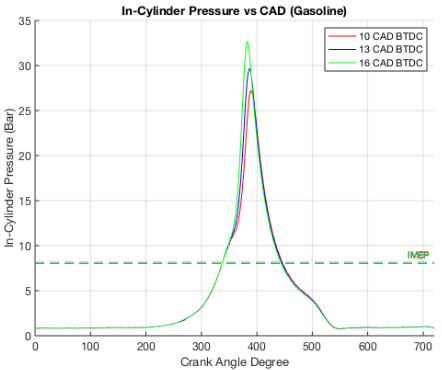
\includegraphics[height = 7cm]{./img/diagram8.png}
    \caption{Variation of in-cylinder pressure against crank angle degree for different spark timings using gasoline.}
    \label{q1-f1}
\end{figure}
\begin{figure}[H]
    \centering
    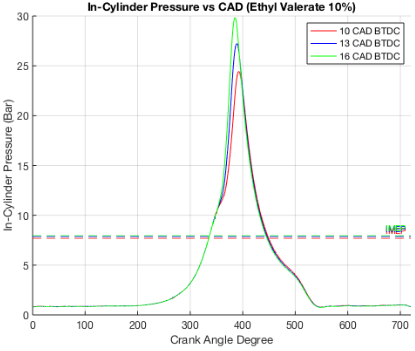
\includegraphics[height = 7cm]{./img/diagram9.png}
    \caption{Variation of in-cylinder pressure against crank angle degree for different spark timings using 10\% Ethyl Valerate.}
    \label{q1-f2}
\end{figure}
While calculating the heat release trace, the following assumptions are made.
\begin{itemize}
    \item Cylinder contents are at a uniform instantaneous temperature (T).
    \item No mass flow occurs across system boundaries.
    \item System is adiabatic.
    \item The cylinder content behaves like an ideal gas.
\end{itemize}
Based on the second law of thermodynamics:
\begin{equation}
    Q_n = Q_{ch} - Q_{ht}
\end{equation}
Where, $Q_n$ is the net apparent heat release, $Q_{ch}$ is the gross heat release of the fuel during combustion and $Q_{ht}$ is the heat transfer from the system to the cylinder walls (negligible). Taking the derivative with respect to CAD, applying the first law of thermodynamics, and using ideal gas law the final equation is derived:
\begin{align}
    \frac{\dif Q_{n}}{\dif \phi} &= \frac{\gamma}{\gamma - 1}\cdot p\cdot \frac{\dif V}{\dif \phi} + \frac{1}{\gamma - 1} \cdot V \cdot \frac{\dif p}{\dif \phi}\\
    \frac{\dif p}{\dif \phi} &= \frac{p_{n+1}-p_n}{\dif \phi}\\
    \frac{\dif V}{\dif \phi} &= \frac{V_{n+1}-V_n}{\dif \phi}
\end{align}
$\gamma = 1.35$ during compression stroke and 1.28 during expansion stroke.

For both gasoline and 10\% ethyl-valerate the heat release trace has been plotted against CAD  for different spark timings with a smoothed line, respectively in Figure \ref{q1-f3} and Figure \ref{q1-f4}. 
\begin{figure}[H]
    \centering
    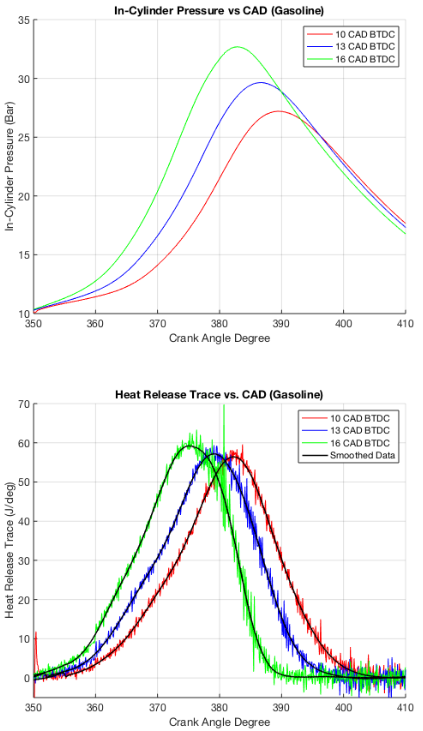
\includegraphics[height = 14cm]{./img/diagram10.png}
    \caption{Calculated and smoothed data for heat release trace for different spark timings using gasoline(b) and in-cylinder pressure values in the corresponding CAD(a).}
    \label{q1-f3}
\end{figure}
\begin{figure}[H]
    \centering
    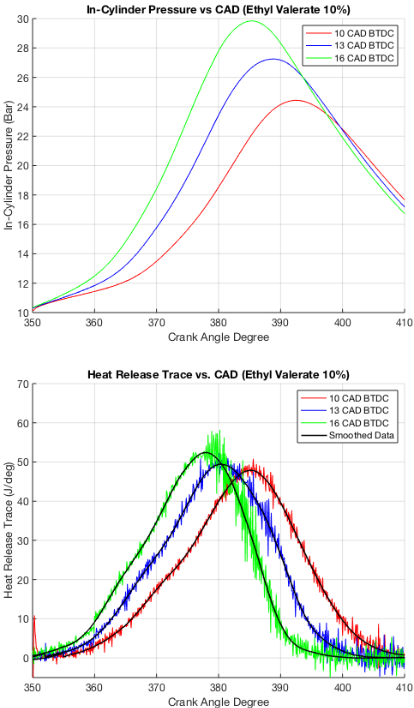
\includegraphics[height = 14cm]{./img/diagram11.png}
    \caption{Calculated and smoothed data for heat release trace for different spark timings using 10\% Ethyl-Valerate(b) and in-cylinder pressure values in the corresponding CAD(a).}
    \label{q1-f4}
\end{figure}
\subsection*{Indicated mean effective pressure (IMEP)}
The indicated mean effective pressure is defined as indicated displacement work per cycle over swept volume of the cylinder: 
\begin{equation}
    \textrm{IMEP} = \frac{W_i}{V_d}
\end{equation}
Where, 
$W_i = \int \left(p\right)\dif V$ and $V_d = \SI{506.8}{\centi\meter\cubed}$ as stated in the Ricardo E6 engine specification \cite{r0}. $W_i$ is calculated using the “trapz” function in MATLAB, and the variation of IMEP for different spark timings are plotted for both fuel content in Figure \ref{q1-f5}. 
\begin{figure}[H]
    \centering
    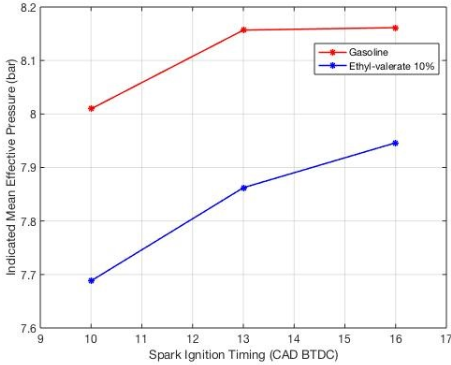
\includegraphics[height = 7cm]{./img/diagram12.png}
    \caption{Variation of IMEP against spark ignition timing for both fuels.}
    \label{q1-f5}
\end{figure}
\subsection*{Apparent net peak heat release rate and crank angle degree at which the apparent net peak heat release rate occurs.}
The apparent net peak heat release rate and the corresponding CAD is taken from the smoothed data in Figure \ref{q1-f6}, to eliminate any noise related error. The apparent net peak release rate variation for different spark timing can be seen in Figure \ref{q1-f7}, and the CAD variation can be seen in Figure \ref{q1-f8}.
\begin{figure}[H]
    \centering
    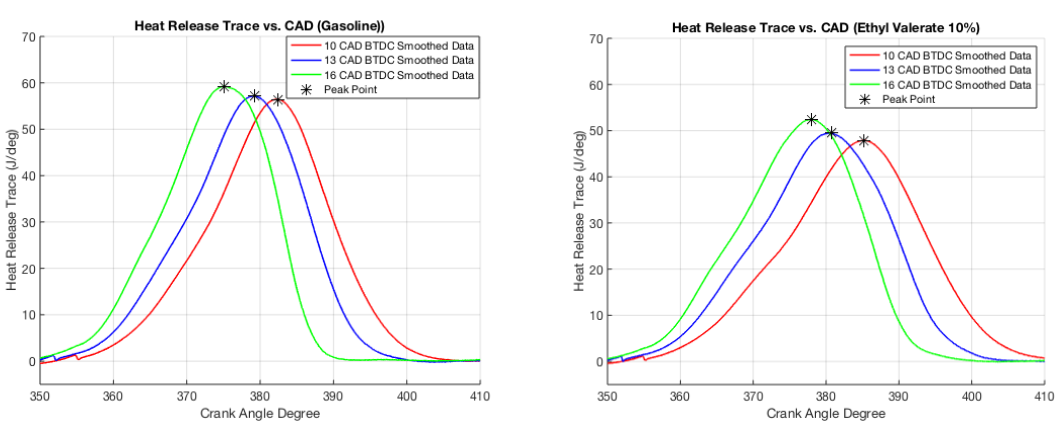
\includegraphics[width = \textwidth]{./img/diagram13.png}
    \caption{Peak points of heat release trace in smoothed data for different spark timings, for Gasoline(a) and Ethyl-valerate (b).}
    \label{q1-f6}
\end{figure}
\begin{figure}[H]
    \centering
    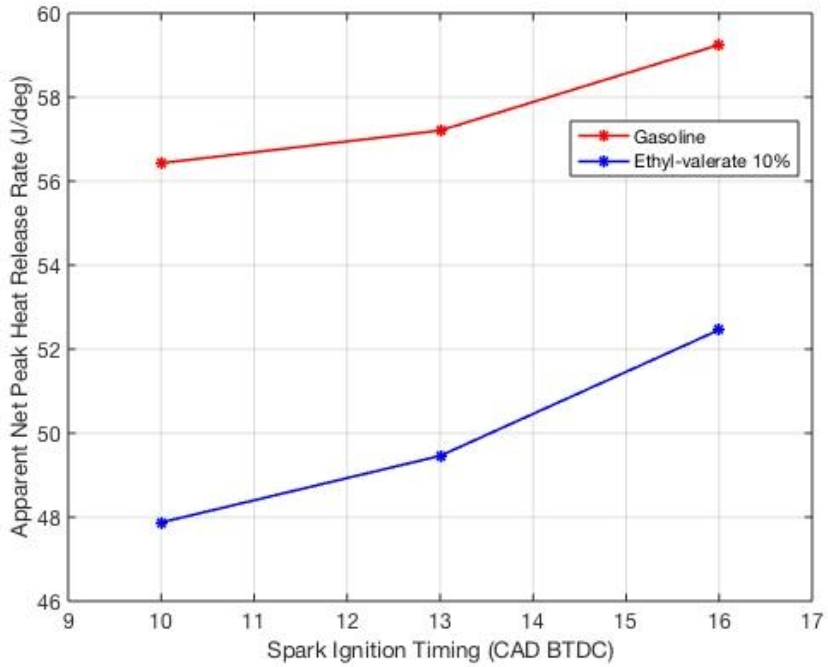
\includegraphics[height = 7cm]{./img/diagram14.png}
    \caption{Variation of apparent net peak heat release rate against spark ignition timing for both fuels.}
    \label{q1-f7}
\end{figure}
\begin{figure}[H]
    \centering
    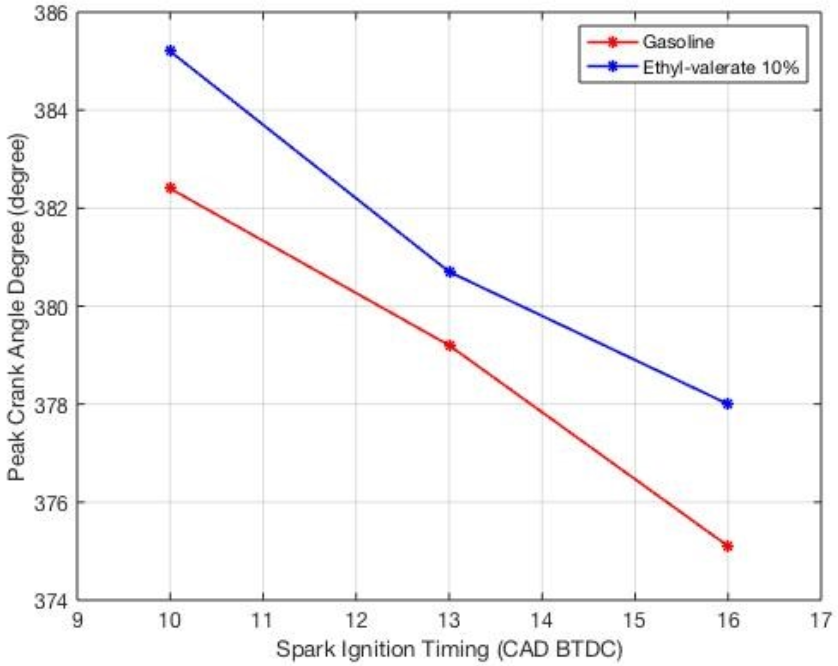
\includegraphics[height = 7cm]{./img/diagram15.png}
    \caption{Variation of CAD at which apparent net peak heat release rate occurs against spark ignition timing for both fuels.}
    \label{q1-f8}
\end{figure}
\begin{table}[H]
    \begin{center}
    \begin{tabular}{@{}l l l l l@{}}
        \toprule
        \multicolumn{5}{c}{\textbf{Gasoline}}\\
        Spark time & Tests & IMEP (bar) & Apparent net peak heat & Crank angle degree\\
        & & & release rate (\si{\joule}/deg) & at peak (deg)\\
        \midrule
        10 CAD  & Test 1    & 7.9708    & 57.8557   & 382.0\\
        BTDC    & Test 2    & 8.0227    & 56.1861   & 382.8\\
                & Test 3    & 8.0352    & 55.4070   & 382.8\\
                & Average   & 8.0096    & 56.4286   & 382.4\\
        13 CAD  & Test 4    & 8.1531    & 56.8654   & 379.2\\
        BTDC    & Test 5    & 8.1795    & 56.7089   & 379.0\\
                & Test 6    & 8.1378    & 58.0777   & 378.8\\
                & Average   & 8.1568    & 57.2049   & 379.2\\
        16 CAD  & Test 7    & 8.1665    & 58.6862   & 379.2\\
        BTDC    & Test 8    & 8.1586    & 59.4184   & 375.1\\
                & Test 9    & 8.1590    & 60.1389   & 375.8\\
                & Average   & 8.1614    & 59.2449   & 375.1\\
        \bottomrule
    \end{tabular}
    \caption{Table showing IMEP, apparent net peak heat release rate and corresponding crank angle degree, for gasoline.}
    \label{q1-t1}
\end{center}
\end{table}
\begin{table}[H]
    \begin{center}
    \begin{tabular}{@{}l l l l l@{}}
        \toprule
        \multicolumn{5}{c}{\textbf{Ethyl-Valerate 10\%}}\\
        Spark time & Tests & IMEP (bar) & Apparent net peak heat & Crank angle degree\\
        & & & release rate (\si{\joule}/deg) & at peak (deg)\\
        \midrule
        10 CAD  & Test 10   & 7.7599    & 49.9627   & 385.2\\
        BTDC    & Test 11   & 7.6285    & 49.1097   & 385.9\\
                & Test 12   & 7.6755    & 46.8893   & 385.0\\
                & Average   & 7.6880    & 47.8727   & 385.2\\
        13 CAD  & Test 13   & 7.8717    & 49.4222   & 381.2\\
        BTDC    & Test 14   & 7.8310    & 48.2018   & 380.1\\
                & Test 15   & 7.8839    & 50.8594   & 380.5\\
                & Average   & 7.8622    & 49.4592   & 380.7\\
        16 CAD  & Test 16   & 7.8919    & 50.6153   & 377.7\\
        BTDC    & Test 17   & 7.9554    & 52.6286   & 378.5\\
                & Test 18   & 7.9909    & 54.2366   & 378.0\\
                & Average   & 7.9460    & 52.4592   & 378.0\\
        \bottomrule
    \end{tabular}
    \caption{Table showing IMEP, apparent net peak heat release rate and corresponding crank angle degree, for Ethyl-Valerate 10\%.}
    \label{q1-t2}
\end{center}
\end{table}
Looking at Tables \ref{q1-t1} and \ref{q1-t2}, both gasoline and 10\% ethyl-valerate seems to have similar trend in every calculated variable.  As seen from Figure \ref{q1-f1} and \ref{q1-f2}, the average in-cylinder pressures increase in amplitude and the peak shifts towards left with earlier spark ignition time, which also results in increasing IMEP, highlighted in Figure \ref{q1-f5}. The same trends can also be seen in the heat release trace plots in Figure \ref{q1-f6}.  

These results are expected as earlier spark ignition time would result in earlier combustion of the fuel, which decreases the CAD at which net peak heat release rate and pressure occurs, resulting in a shift towards left. Furthermore, the early ignition results in higher average in-cylinder pressure, and thus higher IMEP. This may be due to most of the combustion happening near TDC as the spark timing advances BTDC. As the combustion occurs closer to TDC, more of the product gas will expand and increase the work output on the piston by pushing it down. The peak pressure at the combustion closer to TDC therefore will be higher as it will occur in lower cylinder volume. However, if the spark timing is too early and the combustion happens as the piston is rising before TDC, the performance will drop significantly \cite{q1-r1}. Moreover, as the heat release trace depends on in-cylinder pressure, the apparent net peak release rate is higher in earlier ignition time. The higher pressure increase rate in earlier ignition time causes more heat to be released faster \cite{q1-r2}. 

Comparing the fuels, gasoline has higher overall IMEP and Apparent net peak release rate than 10\% ethyl-valerate, seen respectively from Figure \ref{q1-f5} and Figure \ref{q1-f7} Moreover, the peak CAD was earlier in gasoline than that of ethyl-valerate, seen in Figure \ref{q1-f8}. As IMEP is directly related with work done on the piston, it is safe to say that gasoline has better performance compared to 10\% ethyl-valerate. 

The MATLAB code may be viewed online at the following link: \url{https://github.com/hashadar/ME-Latex/tree/master/MECH0011/Renewable%20Fuels%20Lab}
\section{Question 2}
\subsection*{Average emissions of \ce{CO}, \ce{CO2}, \ce{NO_x}}
In order to calculate the average \ce{CO2} and \ce{NO_x} emissions, the emission data acquired from the sensors are plotted against time for every test. When possible, the stable region with low variance is selected to average the emissions. The calculated \ce{CO2} and \ce{NO_x} emission means for each test and average of each spark ignition time can be seen in Table \ref{q2-t1} and \ref{q2-t2}.
\begin{table}[H]
    \begin{center}
    \begin{tabular}{@{}l l l l@{}}
        \toprule
        \multicolumn{4}{c}{\textbf{Gasoline}}\\
        Spark time & Tests & \ce{CO2} emission & \ce{NO_x} emission\\
        & & concentration (\%) & concentration (ppm) \\
        \midrule
        10 CAD  & Test 1    & 14.4167   & 3162  \\
        BTDC    & Test 2    & 14.4311   & 3155  \\
                & Test 3    & 14.4815   & 3110  \\
                & Average   & 14.4331   & 3142  \\
        13 CAD  & Test 4    & 14.4167   & 3162  \\
        BTDC    & Test 5    & 14.4732   & 3246  \\
                & Test 6    & 14.7239   & 2799  \\
                & Average   & 14.7197   & 2781  \\
        16 CAD  & Test 7    & 14.6996   & 751  \\
        BTDC    & Test 8    & 14.6944   & 243  \\
                & Test 9    & 14.6778   & 146  \\
                & Average   & 14.6906   & 380  \\
        \bottomrule
    \end{tabular}
    \caption{\ce{CO2} and \ce{NO_x} emissions for gasoline.}
    \label{q2-t1}
\end{center}
\end{table}
\begin{table}[H]
    \begin{center}
    \begin{tabular}{@{}l l l l@{}}
        \toprule
        \multicolumn{4}{c}{\textbf{Ethyl Valerate 10\%}}\\
        Spark time & Tests & \ce{CO2} emission & \ce{NO_x} emission\\
        & & concentration (\%) & concentration (ppm) \\
        \midrule
        10 CAD  & Test 10    & 13.5300   & 2916  \\
        BTDC    & Test 11    & 13.5463   & 2192  \\
                & Test 12    & 13.5418   & 1126  \\
                & Average    & 13.5394   & 2079  \\
        13 CAD  & Test 13    & 13.5274   & 98  \\
        BTDC    & Test 14    & 13.5229   & 48  \\
                & Test 15    & 13.5183   & 31  \\
                & Average    & 13.5229   & 56  \\
        16 CAD  & Test 16    & 13.4397   & 20  \\
        BTDC    & Test 17    & 13.4464   & 14  \\
                & Test 18    & 13.4266   & 13  \\
                & Average    & 13.4556   & 16  \\
        \bottomrule
    \end{tabular}
    \caption{\ce{CO2} and \ce{NO_x} emissions for Ethyl-Valerate.}
    \label{q2-t2}
\end{center}
\end{table}
\begin{figure}[H]
    \centering
    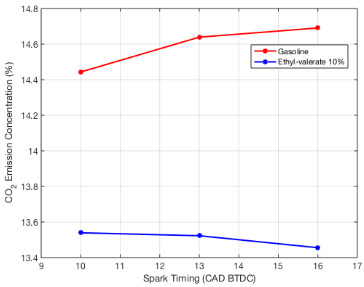
\includegraphics[height = 7cm]{./img/diagram4.png}
    \caption{\ce{CO2} emissions plotted for varying spark ignition timings for both fuels.}
    \label{q2-f1}
\end{figure}
\begin{figure}[H]
    \centering
    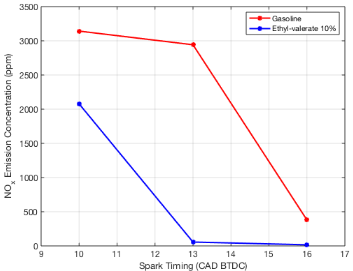
\includegraphics[height = 7cm]{./img/diagram5.png}
    \caption{\ce{NO_x} emissions plotted for varying spark ignition timings for both fuels.}
    \label{q2-f2}
\end{figure}
Looking at Figure \ref{q2-f1}, it is very clear that as the sparking time increased, gasoline showed an increasing \ce{CO2} emission trend while the ethyl-valerate had a decreasing trend; the \ce{CO2} emission for gasoline peaked at 16 CAD BTDC where the latter peaked at 10 CAD BTDC. In addition, it should be noted that gasoline always had a larger emission of \ce{CO2} than ethyl-valerate from 10 to 16 CAD. 

As shown in Figure \ref{q2-f2}, through out the tests gasoline had higher emissions of \ce{NO_x} compared to ethyl-valerate. Unlike \ce{CO2} emissions, both gasoline and ethyl-valerate gave a similar response for \ce{NO_x} emissions as emissions for both decreased with earlier spark ignition timing. On the other hand, the emission of \ce{NO_x} for gasoline had a significant drop between 13 and 16 CAD BTDC while the ethyl-valerate experienced a drastic decline between 10 to 13 CAD BTDC. The \ce{NO_x} emissions for ethyl-valerate between 13 and 16 CAD BTDC is comparatively lower than any other value. 

Overall, as highlighted in Figure \ref{q2-f1} and \ref{q2-f2}, gasoline consistently had significantly larger emission of both \ce{NO_x} and \ce{CO2}  between 10 to 16 CAD BTDC, this phenomenon can be explained by the greater number of carbons in gasoline; the molecular formula of ethyl-valerate is \ce{C7H14O2} \cite{q2-r1} and the main component of gasoline is octane, which has a molecular formula of \ce{C8H18} \cite{q2-r2}. Greater number of carbons means more \ce{CO2} would be produced and larger amount of oxygen is required, since the formation of \ce{NO_x} is highly temperature and \ce{O2} concentration dependent, high temperatures and \ce{O2} concentrations will result in high \ce{NO_x} formation rate. As more oxygen is obtained during the chemical reaction of air with gasoline than the reaction of air with ethyl-valerate, more \ce{NO_x} is released by gasoline \cite{q2-r3}.
\subsection*{Peak heat release rate}
\begin{figure}[H]
    \centering
    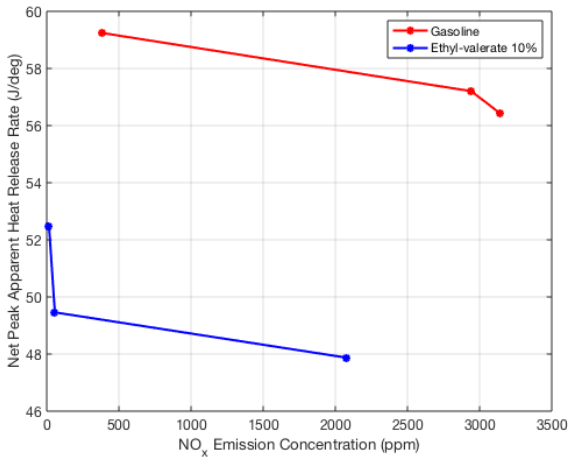
\includegraphics[height = 7cm]{./img/diagram6.png}
    \caption{Plot of net peak heat release rate against \ce{NO_x} emissions for both fuels.}
    \label{q2-f3}
\end{figure}
\begin{figure}[H]
    \centering
    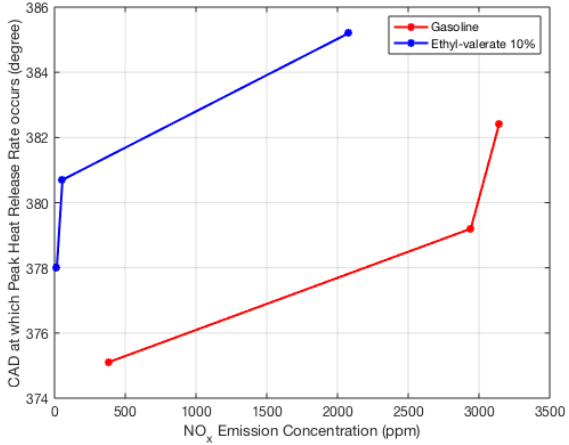
\includegraphics[height = 7cm]{./img/diagram7.png}
    \caption{Plot of CAD at which peak heat release rate occurs against \ce{NO_x} emissions for both fuels.}
    \label{q2-f4}
\end{figure}
Theoretically, \ce{NO_x} emissions should increase as the peak heat release rate rises. As described previously, high temperature, pressure, and oxygen concentration would result in higher \ce{NO_x} formation rate and therefore higher emissions. However, results shown in Figure \ref{q2-f3} give a completely opposite response, the emission of \ce{NO_x} for both gasoline and ethyl-valerate showed a tendency to decrease as the peak heat release rate increased.  

There are a few errors that could have caused errors in calculations.
\begin{enumerate}
    \item In calculations, the assumptions of a perfectly adiabatic system and stoichiometric combustions are made. However, in reality the system is not perfect and there are frictional and environmental heat losses. 
    \item As mentioned previously, as the emissions are recorded with respect to time, emissions are averaged in a stable region when possible. However, emissions didn’t reach equilibrium for all tests and were unstable across the cycle. In some of the tests, emissions data displayed decreasing trend over time and didn’t become steady. As seen from Table \ref{q2-t1}, for some spark ignition time tests, there are significant cycle-to-cycle variations in emissions. For more accurate data, more tests with a steady emission level should be conducted. 
    \item It is possible that the measuring instrument used to detect \ce{NO_x} and \ce{CO2} emissions may have errors, especially calibration error.
    \item The heat released may not be uniformly distributed, which makes the measurement inaccurate and leads to deviations from the calculated values. 
\end{enumerate}
\section{Question 3}
The lower heating value is the amount of heat released in the complete combustion of a specific quantity of fuel at standard conditions (\SI{25}{\celsius} and \SI{1}{\bar}), without recovering the latent heat of vaporization from the water vapour content in the gaseous products \cite{q3-r1}. The LHV is preferred to HHV in relation to internal combustion engines as it is not practical to recover the energy contained in the gaseous water vapour in typical ICEs, as this would require cooling the combustion products until the water vapour condenses. In most engines the vapour is expelled from the system as part of the hot exhaust gases and is therefore unavailable to do useful work. 

Heating values may be determined using a calorimeter or derived empirically by considering an energy balance, as will be done here. The heating value of the renewable fuel, ethyl valerate (\ce{C7H14O2}), was estimated by considering its stoichiometric combustion in dry air. The chemical equation is presented as follows: 
\begin{equation}
    \ce{C7H14O2 + 9.5(O2 + 3.76N2) -> 7CO2 + 7H2O(g) + 35.72N2} \label{q3-1}
\end{equation}
Assuming perfect homogenous mixing of fuel and air, \SI{9.5}{\mol} of dry air (21\% oxygen and 79\% nitrogen by volume) is required per mole of fuel to achieve complete combustion. The heat released is therefore the difference between the enthalpies of the products and reactants \cite{q3-r2}.
\begin{equation}
    Q = \sum_P \left(n_i\overline{h_i}\right) - \sum_R \left(n_i\overline{h_i}\right) = H_P - H_R \label{q3-2}
\end{equation}
The enthalpy $\overline{h_i}$ at any state is a function of temperature and pressure, consists of the enthalpy of formation $h_f^{\ominus}$ at standard reference conditions and sensible enthalpy. For simplicity, only the enthalpy of formation was considered in the estimation as the exhaust temperatures are not known. This causes the heat release to be overestimated and leads to conservative results for thermal efficiency. 

According to the National Institute of Standards and Technology, the enthalpy of formation of the test fuel is $\Delta h_f^{\ominus} = \SI{-553}{\kilo\joule\per\mol}$ \cite{q3-r3}. $h_f^{\ominus}$ of the other compounds were obtained from property tables \cite{q4-r4}. From \eqref{q3-1} and \eqref{q3-2}, the LHB of ethyl valerate (\ce{C7H14O2}) is computed as follows:
\begin{equation}
    LHV_{\textrm{test}} = \left[-553.1-9.5\left(0+0\right)\right]-\left[7\left(-393.52\right)+7\left(-241.82\right)+35.72\left(0\right)\right] = \SI{3894.4}{\kilo\joule\per\mol}
\end{equation}
Taking the molecular weight of ethyl valerate to be \SI{130.185}{\kilo\gram\per\mole}, the LHV of the test fuel expressed in mass basis is: 
\begin{equation}
    LHV_{\ce{C7H14O2}} = \SI{29.91}{\mega\joule\per\kg}
\end{equation}
The LHV of the reference fossil gasoline is as provided: 
\begin{equation}
    LHV_{\textrm{G}} = \SI{42.7}{\mega\joule\per\kg}
\end{equation}
Therefore, the LHV of the fuel blend is the sum of the LHVs of the ethyl valerate and gasoline, weighted by mass fractions ($x_i$), which can be computed from their volume fractions ($v_i$). \cite{q3-r1}
\begin{align}
    LHV_{\textrm{blend}} &= x_G \cdot \left(LHV\right)_G + x_{\ce{C7H14O2}} \cdot \left(LHV\right)_{\ce{C7H14O2}}\\
    x_G &= \frac{v_G \rho_G}{v_G \rho_G + v_{\ce{C7H14O2}}\rho_{\ce{C7H14O2}}}\\
    \therefore LHV_{\textrm{blend}} &= 0.88267\left(42.7\right) + \left(1-0.88267\right)\left(29.913\right) = \SI{41.20}{\mega\joule\per\kg}
\end{align}
The indicated specific fuel consumption ISFC is a measure of the amount of fuel used per unit of power output from the engine. It is given by the following equation \cite{q3-r5}
\begin{equation}
    ISFC = \frac{\dot{m}_f}{\dot{W}} \label{q3-3}
\end{equation}
Where $\dot{m}_f$ is the mass flow rate of fuel and $\dot{W}$ is the power output. The power output of the engine may be derived from the indicated mean effective pressure IMEP calculated in Question 1, which is the average pressure required in the cylinder to produce the same amount of work throughout the 4 strokes. As IMEP does not factor friction losses, the power output is overestimated hence the actual fuel consumption is higher. The work done per power stroke is expressed as: 
\begin{equation}
    W_{\textrm{power}} = IMEP \times \textrm{Bore Area} \times \textrm{Stroke} = IMEP \times \textrm{Swept volume} \label{q3-4}
\end{equation}
The Ricardo E6 is a 4-stroke engine running at test conditions of 600 rpm, therefore there is 1 power stroke every 2 crankshaft rotations, i.e. 5 power strokes per second. The power output in \si{\kilo\watt} is:
\begin{equation}
    \dot{W} = 5\dot{W}_{\textrm{power}} \label{q3-5}
\end{equation}
The overall indicated thermal efficiency for the engine is by definition the useful work output over total heat input. It is a measure of how much of the fuel’s heating value is lost to incomplete combustion, heat loss to surroundings and friction, and other losses. Taking the cylinder to be the system, the heat input is simply the heat released during combustion within the cylinder, equal to mass flow rate of fuel times the fuel heating value. 
\begin{equation}
    \eta_{th} = \frac{\dot{W}}{\dot{Q}_{in}} = \frac{\dot{W}}{\dot{m}_f \times LHV_{\textrm{blend}}} \label{q3-6}
\end{equation}
Therefore, the efficiency and ISFC are related by the following: 
\begin{equation}
    \eta_{th} = \frac{1}{ISFC \times LHV_{\textrm{blend}}}
\end{equation}
Using the above relations, the calculated values for ISFC and indicated thermal efficiency for each spark timing are presented in Table \ref{q3-t1}, with the corresponding IMEP for reference. The thermal efficiencies were plotted against spark timing in Figure \ref{q3-f1}.
\begin{table}[H]
    \begin{center}
    \begin{tabular}{@{}l l l l l@{}}
        \toprule
        Fuel & Spark time &IMEP (\si{bar}) & Indicated specific fuel & Indicated thermal \\
        & (deg BTDC) & & consumption (\si{\kg\per\joule}) & efficiency\\
        \midrule
        Reference   & 10    & 8.0096    & \SI{8.0218e-8}    & 0.292\\
        fossil      & 13    & 8.1568    & \SI{7.7742e-8}    & 0.302\\
        gasoline    & 16    & 8.1614    & \SI{7.8758e-8}    & 0.297\\
        \midrule
        10\% Ethyl  & 10    & 7.6880    & \SI{7.8958e-8}    & 0.307\\
        valerate    & 13    & 7.8622    & \SI{7.8158e-8}    & 0.311\\
                    & 16    & 7.9461    & \SI{7.6111e-8}    & 0.319\\
        \bottomrule
    \end{tabular}
    \caption{ISFC consumptions and indicated thermal efficiencies.}
    \label{q3-t1}
    \end{center}
\end{table}
\begin{figure}[H]
    \centering
    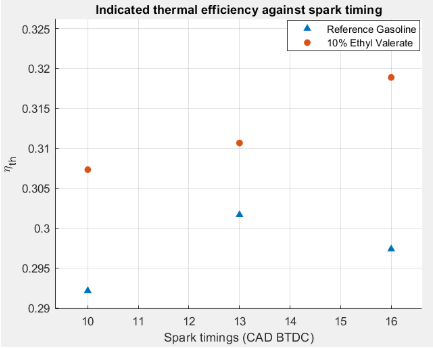
\includegraphics[height = 7cm]{./img/diagram1.png}
    \caption{Plot of indicated thermal efficiency against spark timing}
    \label{q3-f1}
\end{figure}
It is observed that thermal efficiency of the engine running on the fuel blend is higher than that of gasoline at all spark timings. Although the engine produces less work on the blend, the heat input requirements are also lower. 

The trend shows that in general, the indicated thermal efficiency increases with retarded spark timings. This is to be expected as earlier spark timings resulted in higher IMEPs, which translates to a higher indicated power output. Spark timings that are too advanced result in the gas expanding when the piston is already moving down from TDC, hence work done by the gas is not maximised. However, if the spark timing is too early, the gas expands against the piston when it is moving up towards TDC and it is not doing useful work. It has been determined experimentally that optimal power and efficiency for a spark ignition gasoline engine is achieved at 31 CAD BTDC (Zareei and Kakaee, 2013) \cite{q1-r1}. Therefore, for the range investigated in this experiment, an increase in indicated thermal efficiency with spark timing was expected to be observed.

For this reason, the efficiency for the gasoline fuel at 13 or 16 CAD BTDC was most likely to be anomalous as it does not fit with expectations of the trend. Although the IMEP showed a linear increase with later spark timings, the ISFC of the 13 CAD BTDC trial was significantly lower than 16 CAD BTDC. The reason for this anomaly can possibly be attributed to the measured fuel flow rate during test 4, which ranged from \SI{0.18}{\gram\per\second} at the beginning of the test to \SI{0.1}{\gram\per\second} by the end, giving a lower average fuel flow rate compared to the other two tests ran at the same spark timing. Since air mass flow rate remained relatively constant, and the methodology called for the air fuel ratio to remain constant throughout, this must be the result of an error, human or otherwise. This thus increased the average ISFC and thermal efficiency of the gasoline at 13 CAD BTDC. Removing the results of test 4 gives us a revised thermal efficiency closer to 29.6\%, which is much more reasonable given the expected trend. The revised thermal efficiencies with test 4 removed were plotted against spark timing in Figure \ref{q3-f2}. 
\begin{figure}[H]
    \centering
    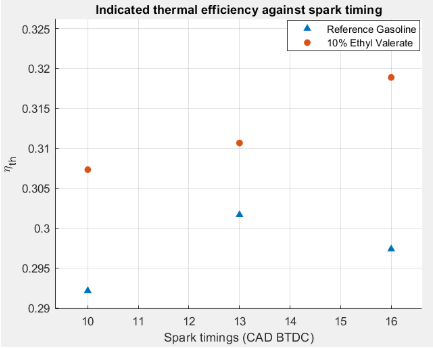
\includegraphics[height = 7cm]{./img/diagram1.png}
    \caption{Plot of indicated thermal efficiency with test 4 removed.}
    \label{q3-f2}
\end{figure}
In general, the LHV is an inaccurate estimate for heat input to the system. As mentioned previously the estimated LHV of the fuel blend overestimates the heat released in its combustion, hence the thermal efficiency is likely underestimated. Furthermore, using the product of fuel mass flow and LHV as $Q_{in}$ assumes that perfect combustion occurs, and the fuel is burnt completely. In reality, there will not be a homogenous mixture of air and fuel, hence there will be pockets of unburnt fuel that leave in the exhaust gases. In this manner, $Q_{in}$ is again overestimated.  

Additionally, as mentioned previously since the power output is an overestimate, since it was derived from the IMEP which this does not consider frictional losses which may occur in the moving parts of an ICE. Hence, the useful power will be lower in practical purposes and thus the thermal efficiencies calculated are also an overestimate. 

Lastly, it is important to consider whether it is appropriate to evaluate the system using thermodynamic analysis. Thermodynamic efficiency of the spark ignition engine is derived from the closed system analysis of the Otto cycle, whilst our experiment deals with a system that undergoes a mechanical cycle instead of a thermodynamic one. Though thermodynamic analysis is not strictly accurate with regards to our system, it is still useful for observing trends within our data. Our analysis allows us to conclude that efficiency increases with increased spark timings, and for all spark timings, the ethyl valerate fuel blend yields a higher thermal efficiency, meaning more energy is converted to useful work.  
\section{Question 4}
Applying the First Law to the Internal Combustion Engine, we get the following sources of energy inputs and outputs to the system as shown in Figure \ref{q4-f1}. Table \ref{q4-t1} shows the amount of energy each category comprises, for each of the tests, which are then plotted in Figures \ref{q4-f6} and \ref{q4-f7}. The energy balance is:
\begin{equation}
	Q_\textrm{ch} = W_\textrm{i} + Q_\textrm{ex} + Q_\textrm{ht} + Q_\textrm{other}\label{q4-1}
\end{equation}
\begin{itemize}
	\item $Q_\textrm{ch}$ is the gross heat release of fuel during combustion.
	\item $W_\textrm{i}$ is the indicated displacement work output (cylinder power output).
	\item $Q_\textrm{ex}$ is the energy to engine exhaust.
	\item $Q_\textrm{ht}$ is the heat transfer from the system to the cylinder walls (which are transferred as heat to the engine cooling water).
	\item $Q_\textrm{other}$ includes all other sources of energy loss (noise, vibration, heat transfer to surrounding air, etc.).
\end{itemize}
\begin{figure}[H]
	\centering
    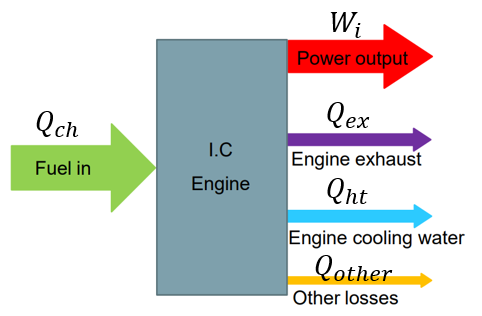
\includegraphics[height = 6cm]{./img/diagram16.png}
    \caption{Energy Balance for I.C. Engine. \cite{r0}}
    \label{q4-f1}
\end{figure}
\begin{figure}[H]
	\centering
    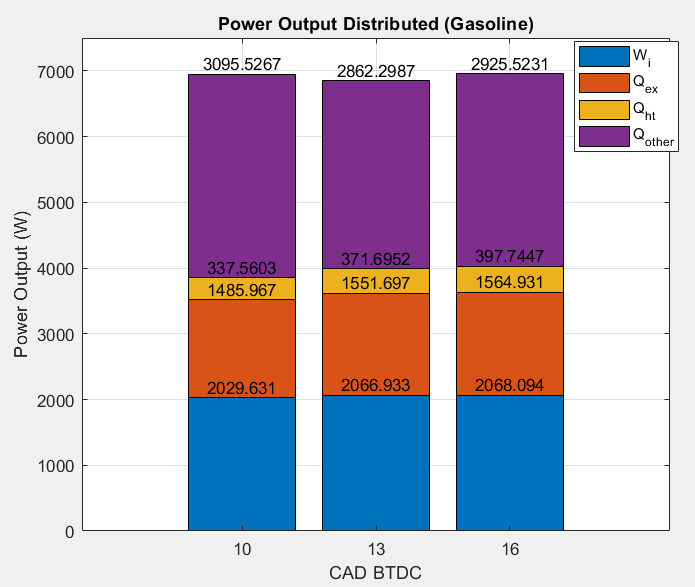
\includegraphics[height = 6cm]{./img/diagram21.png}
    \caption{Proportional Bar Chart (Gasoline)}
    \label{q4-f6}
\end{figure}
\begin{figure}[H]
	\centering
    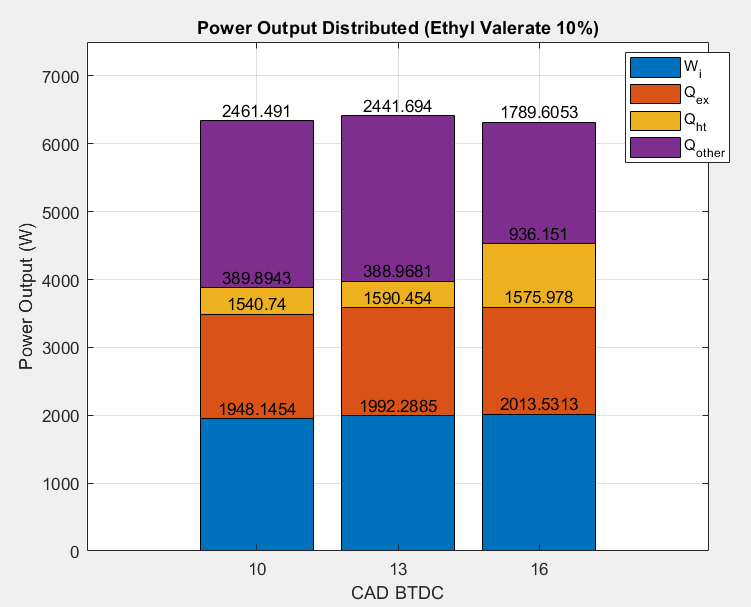
\includegraphics[height = 6cm]{./img/diagram22.png}
    \caption{Proportional Bar Chart (Ethyl-Valerate 10\%)}
    \label{q4-f7}
\end{figure}
\begin{table}[H]
	\begin{center}
	\begin{tabular}{@{}l l l l l l l@{}}
		\toprule
		\multicolumn{7}{c}{\textbf{Gasoline}}\\
		Spark Time & Test & $Q_\textrm{ch}$ (W) & $W_\textrm{i}$ (W) & $Q_\textrm{ex}$ (J/s) & $Q_\textrm{ht}$ (J/s) & Efficiency (\%)\\
		\midrule
				& Test 1  & 6796.5238 & 2019.816 & 1460.246 & 341.1995 & 29.718\\
		10 CAD	& Test 2  & 7048.0320 & 2032.955 & 1483.526 & 322.0532 & 28.844\\
		BTDC	& Test 3  & 7001.4992 & 2036.121 & 1514.127 & 349.4283 & 29.081\\
				& Average & 6948.6850 & 2029.631 & 1485.967 & 337.5603 & 29.215\\
				& Test 4  & 6736.1891 & 2065.986 & 1517.161 & 364.1403 & 30.670\\
		13 CAD	& Test 5  & 6913.5082 & 2072.690 & 1567.170 & 374.9483 & 29.980\\
		BTDC	& Test 6  & 6908.1743 & 2062.123 & 1570.760 & 375.9971 & 29.850\\
				& Average & 6852.6239 & 2066.933 & 1551.697 & 371.6952 & 30.167\\	
				& Test 7  & 6930.5932 & 2069.393 & 1556.818 & 392.0714 & 29.859\\
		16 CAD	& Test 8  & 6834.3491 & 2067.397 & 1557.887 & 397.0891 & 30.250\\
		BTDC	& Test 9  & 7103.9362 & 2067.492 & 1580.087 & 404.0736 & 29.103\\
				& Average & 6956.2928 & 2068.094 & 1564.931 & 397.7447 & 29.737\\		
		\bottomrule
	\end{tabular}
	\caption{Table of proportion of chemical energy to various heat and work output from the system for gasoline}
	\label{q4-t1}
	\end{center}
\end{table}
\begin{table}[H]
	\begin{center}
	\begin{tabular}{@{}l l l l l l l@{}}
		\toprule
		\multicolumn{7}{c}{\textbf{Ethyl-Valerate 10\%}}\\
		Spark Time & Test & $Q_\textrm{ch}$ (W) & $W_\textrm{i}$ (W) & $Q_\textrm{ex}$ (J/s) & $Q_\textrm{ht}$ (J/s) & Efficiency (\%)\\
		\midrule
				& Test 10  & 6393.8485 & 1966.3645 & 1531.301 & 405.0180 & 30.754\\
		10 CAD	& Test 11  & 6205.3713 & 1933.0826 & 1536.155 & 391.1557 & 31.152\\
		BTDC	& Test 12  & 6421.5921 & 1944.9890 & 1554.764 & 373.5094 & 30.288\\
				& Average  & 6340.2707 & 1948.1454 & 1540.740 & 389.8943 & 30.731\\
				& Test 13  & 6457.5565 & 1994.6858 & 1591.637 & 424.4467 & 30.889\\
		13 CAD	& Test 14  & 6342.5951 & 1984.3780 & 1586.476 & 362.6769 & 31.287\\
		BTDC	& Test 15  & 6440.0621 & 1997.8018 & 1593.249 & 379.7808 & 31.021\\
				& Average  & 6413.4046 & 1992.2885 & 1590.454 & 388.9681 & 31.066\\	
				& Test 16  & 6225.6571 & 1999.8119 & 1567.919 & 435.6451 & 32.122\\
		16 CAD	& Test 17  & 6294.3904 & 2015.8882 & 1577.852 & 1127.802 & 32.027\\
		BTDC	& Test 18  & 6425.7492 & 2024.8938 & 1582.163 & 1245.007 & 31.512\\
				& Average  & 6315.2656 & 2013.5313 & 1575.978 & 936.151 & 31.887\\		
		\bottomrule
	\end{tabular}
	\caption{Table of proportion of chemical energy to various heat and work output from the system for Ethyl-Valerate 10\%}
	\label{q4-t2}
	\end{center}
\end{table}
\subsection*{Useful Power Output}
The proportion of the chemical energy from the fuel converted to useful (indicated) power is calculated using the IMEP and displacement volume, as mentioned previously in Q3, using Equations \ref{q3-4} and \ref{q3-5}. The results are plotted in Figure \ref{q4-f2}.
\begin{figure}[H]
	\centering
    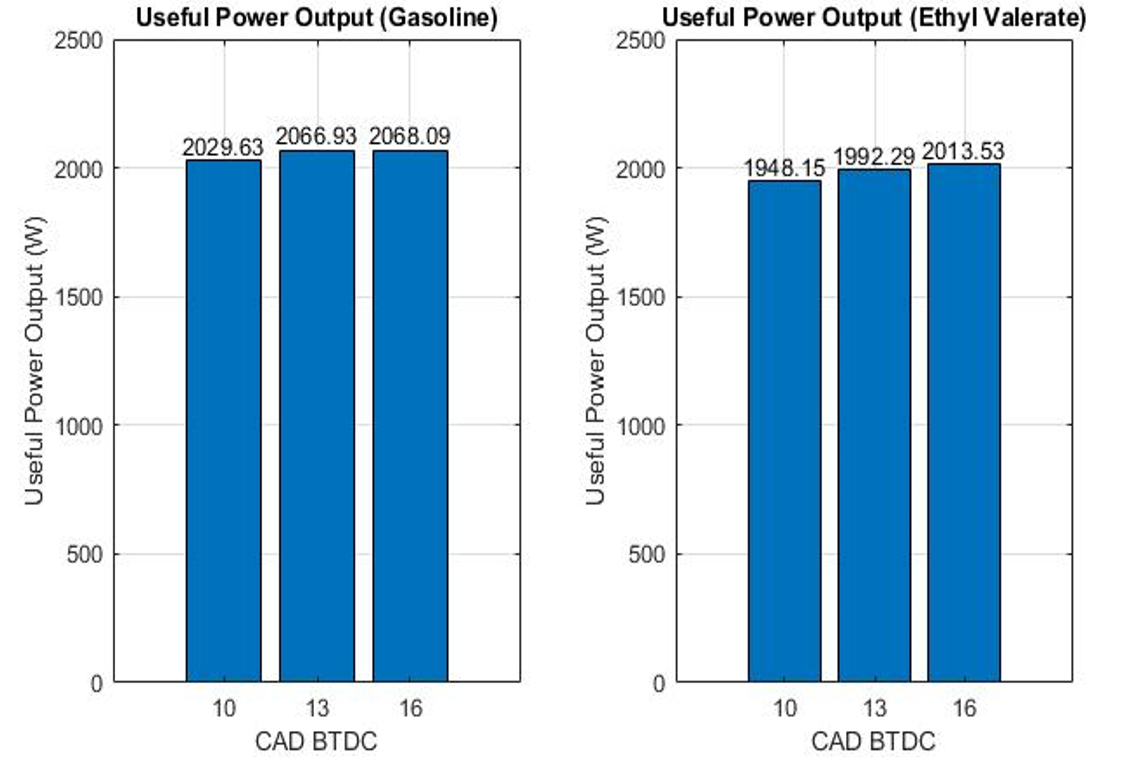
\includegraphics[height = 7cm]{./img/diagram17.png}
    \caption{Bar chart of useful power output for gasoline (left) and Ethyl-Valerate 10\% (right)}
    \label{q4-f2}
\end{figure}
\subsection*{Heat to Cooling Water}
The heat transfer to the cylinder walls is assumed to be perfectly transmitted to the cooling water and responsible for raising its temperature. It was calculated by integrating the heat transfer to the cooling water over the duration of the measurement, using Equation \ref{q4-2}. The results are plotted in \ref{q4-f3}.
\begin{equation}
Q_\textrm{ht} = \frac{\Sigma^{end}_{time step=1} \dot{m}_w \times c_p \times (T_{out} - T_{in}) \times \Delta t}{Duration} \label{q4-2}
\end{equation}
\begin{align*}
\textrm{Where }
\dot{m}_w	&= \textrm{Mass flow rate of engine cooling water (6L/min = 0.1kg/s)}\\
c_p 		&= \textrm{Specific heat capacity of water (\SI{4.18}{\joule\per\gram\per\kelvin})}\\ 
T_{in}		&= \textrm{Temperature of cooling water in}\\ 
T_{out}		&= \textrm{Temperature of cooling water out}\\
\Delta t	&= \textrm{Time step size}
\end{align*}
\begin{figure}[H]
	\centering
    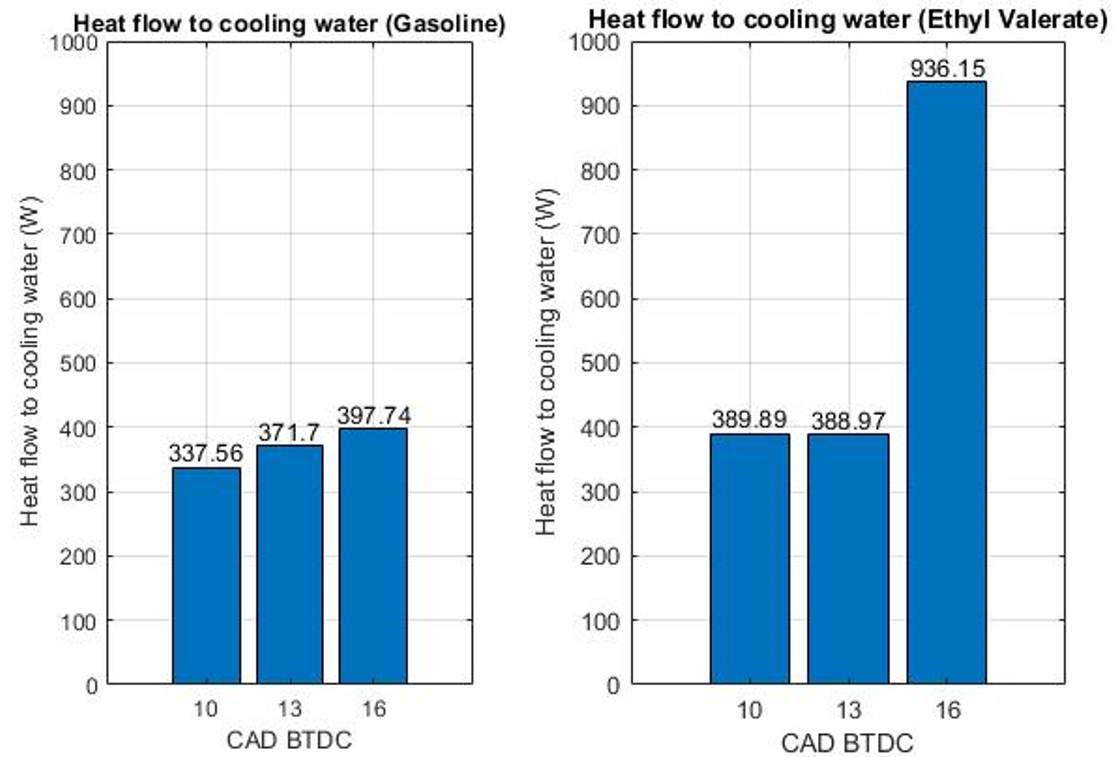
\includegraphics[height = 7cm]{./img/diagram18.png}
    \caption{Bar chart of heat to cooling water for gasoline (left) and Ethyl-Valerate 10\% (right)}
    \label{q4-f3}
\end{figure}
\subsection*{Elevation of Exhaust Gases Temperature}
The heat transferred to the exhaust gases is lost to the system and is unavailable to be converted to work. It is calculated by Equation \ref{q4-3}, and the results plotted in Figure \ref{q4-f4}.
\begin{equation}
Q_{ex} = \dot{m}_{ex} \times c_p \times (T_{out}-T_{in}) \label{q4-3}
\end{equation}
\begin{align*}
\textrm{Where }
\dot{m}_{ex}	&= \dot{m}_{fuel} + \dot{m}_{air} \textrm{ (By conservation of mass)}\\
T_{in}			&= \textrm{Temperature of cooling water in}\\ 
T_{out}			&= \textrm{Temperature of cooling water out}\\
c_p				&= \textrm{Specific heat capacity of exhaust gases, calculated as follows:}
\end{align*}
Making the ideal gas assumption, we can say that the volume fraction is equivalent to mole fraction $y_i$, where $i$ represents all the components of the exhaust gas. Thus the apparent molecular weight of the exhaust gas mixture is:
\begin{equation}
M = \sum\limits_{i=1}^{all} y_i \cdot M_i \label{q4-4}
\end{equation}
The mass fraction of the $i^{th}$ component $x_i$ is given by:
\begin{equation}
x_i= \frac{y_i \cdot M_i}{M} \label{q4-5}
\end{equation}
Therefore, $c_p$ for the exhaust gas is:
\begin{equation}
c_p = \sum \limits_{i=1}^{all} x_i \cdot c_{p,i} \label{q4-6}
\end{equation}
The composition of typical exhaust gases of gasoline engines are as follows in Table \ref{q4-t3}. \cite{q4-r2} \cite{q4-r3} 
\begin{table}[H]
	\begin{center}
	\begin{tabular}{@{}l l l l l l l l@{}}
		\toprule
		Gases & Volume & $y_i$ & $M_i$ & Weighted M & $x_i$ (\%) & $c_p @ 750K$ & Weighted $c_p$ \\
		 & (\%) & (\%) & (g/mol) & (g/mol) & (\%) & (J/g $\textrm{K}^{-1}$) & (J/g $\textrm{K}^{-1}$) \\ 
		\midrule
		\ce{N2} & 71 & 71 & 28.01 & 19.8871 & 66.448 & 1.11 & 0.73757 \\
		\ce{CO2} & 18 & 18 & 44.01 & 7.9218 & 26.469 & 1.148 & 0.30386 \\
		\ce{H2O} & 9.2 & 9.2 & 18.02 & 1.65784 & 5.539 & 2.113 & 0.11704 \\
		\ce{O2} & 0.7 & 0.7 & 32 & 0.224 & 0.748 & 1.043 & 0.00781 \\
		\ce{CO} & 0.85 & 0.85 & 28.01 & 0.238085 & 0.796 & 1.126 & 0.00896 \\
		Others &   &   &   & Negligible &   &   &  \\
		Total & 99.75 & 99.75 & - & 29.929 & 100 & - & 1.17524\\
		\bottomrule
	\end{tabular}
	\caption{Composition of exhaust gases}
	\label{q4-t3}
	\end{center}
\end{table}
\begin{figure}[H]
	\centering
    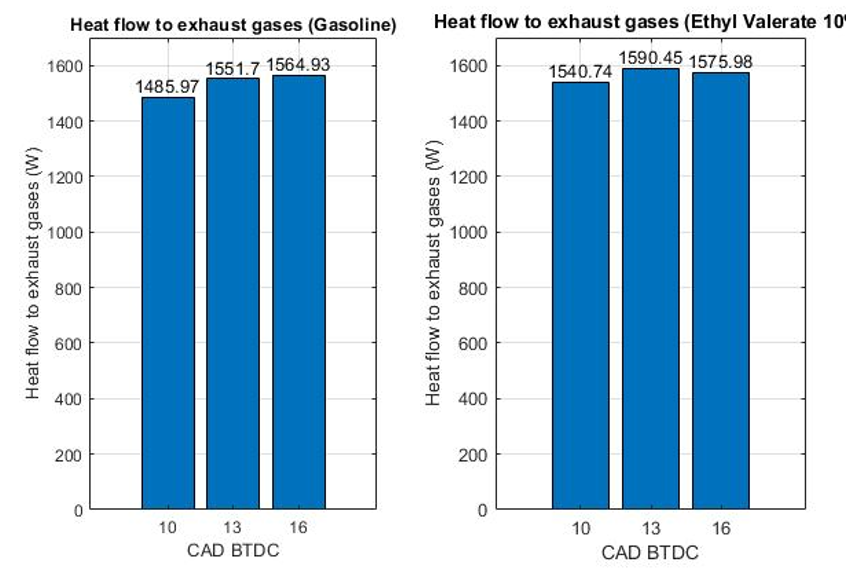
\includegraphics[height = 7cm]{./img/diagram19.png}
    \caption{Bar chart of heat to exhaust gases for gasoline (left) and Ethyl-Valerate 10\% (right)}
    \label{q4-f4}
\end{figure}
\subsection*{Other losses}
Any other losses to the system reduces the amount of energy available to be converted to heat and is undesirable. These may include:
\begin{itemize}
	\item Raising temperature of the engine components/oil.
	\item Heat loss through walls/casing.
	\item Noise and vibrations.
	\item Frictional losses. 
	\item Incomplete combustion - in reality there will not be a homogeneous mixture of air and fuel in the combustion chamber. The pockets of fuel will not get combusted.
	\item Gas leakage from imperfect seal between cylinder piston and walls - there will be loss of cylinder pressure.
\end{itemize}
\subsection*{Discussion}
Firstly, the power calculated is using indicated mean effective pressure. The indicated power does not take frictional losses into account, hence the actual work output is lower. To improve this the break mean effective pressure and break power can be used as it does account for friction losses and hence is a more accurate measure of engine power output. We can also use a torque sensor on the output shaft to measure the actual torque, hence the useful power output would be given by torque multiplied by engine speed (600 RPM).

Secondly, it was observed that from amongst the tests for 16 CAD BTDC for the  Ethyl-Valerate blend, tests 17 and 18 show a dramatically different mass flow rate than test 16 and even all the other tests. As a result, the calculated heat transfer to cooling water is much higher than other tests, as can be seen from Figure \ref{q4-f4}. This may be caused by changing of cooling water flow rate, or the malfunctioning of the sensor. Another possibility is test 16 was not fully preheated or the test 17 and 18 were overheated. More measurements should be taken and ensuring that the cooling water and engine is running in stable status.

Finally, the time step between each measurement data point is not equal, hence Equation \ref{q4-3} to calculate heat going towards elevating the temperature of exhaust gases is inaccurate. The accurate way of calculating energy out should be:
\begin{align*}
Q_{ex} &= \frac{\sum \textrm{Instantaneous } \dot{m}_{ex} \cdot c_p \cdot \Delta T \cdot \textrm{Time Step}}{\textrm{Total Duration}} \\
&= \frac{\sum \limits_{i=1}^{all} \dot{m}_{i} \cdot c_p \cdot (T_i-T_{ambient}) \cdot (t_{n+1}-t_n)}{\textrm{Total Duration}}
\end{align*}
\subsection*{Comparison to theoretical Otto Cycle}
Comparing the Otto Cycle and real case, we notice that the pumping losses is not considered in the cycle (Figure \ref{q4-f5}). The Otto cycle also only consider one rotation as a cycle, which ignore the expansion and compression for exhaust stroke and intake stroke. Thus, the Otto Cycle will have much higher work output. The calculation for Otto cycle is shown below \cite{q4-r4}, and the results are displayed and compared to the experimental in Tables \ref{q4-t4} and \ref{q4-t5}.
\begin{eqnarray}
Q_{in} = W_{output} + Q_{out}\\
Q_{in} = Q_{ch} \textrm{ and } Q_{out} = Q_{ex}\\
W_{output} = Q_{ch} - Q_{ex}
\end{eqnarray}
\begin{figure}[H]
	\centering
    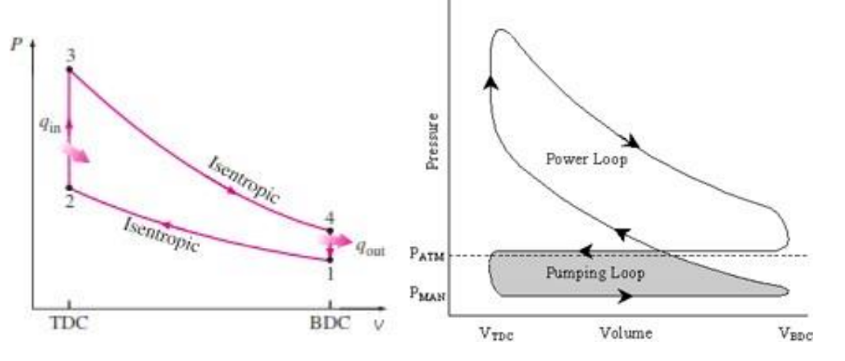
\includegraphics[height = 5cm]{./img/diagram20.png}
    \caption{P-v diagram of Otto Cycle (left) vs. Real Cycle (right)}
    \label{q4-f5}
\end{figure}
\begin{table}[H]
	\begin{center}
	\begin{tabular}{@{}l l l l l l@{}}
		\toprule
		\multicolumn{6}{c}{\textbf{Gasoline}} \\
		Spark Time & Test & $Q_\textrm{ch}$ (W) & $Q_\textrm{ex}$ (J/s) & $W_\textrm{otto}$ (W) & $W_\textrm{exp}$ (W) \\ 
		\midrule
				& Test 1  & 6796.5238 & 1460.246 & 5336.278 & 2019.816\\
		10 CAD	& Test 2  & 7048.0320 & 1483.526 & 5564.506 & 2032.955\\
		BTDC	& Test 3  & 7001.4992 & 1514.127 & 5487.372 & 2036.121\\
				& Average & 6948.6850 & 1485.967 & 5462.718 & 2029.631\\
				& Test 4  & 6736.1891 & 1517.161 & 5219.028 & 2065.986\\
		13 CAD	& Test 5  & 6913.5082 & 1567.170 & 5346.338 & 2072.690\\
		BTDC	& Test 6  & 6908.1743 & 1570.760 & 5337.414 & 2062.123\\
				& Average & 6852.6239 & 1551.697 & 5300.927 & 2066.933\\	
				& Test 7  & 6930.5932 & 1556.818 & 5373.775 & 2069.393\\
		16 CAD	& Test 8  & 6834.3491 & 1557.887 & 5276.462 & 2067.397\\
		BTDC	& Test 9  & 7103.9362 & 1580.087 & 5523.849 & 2067.492\\
				& Average & 6956.2928 & 1564.931 & 5391.362 & 2068.094\\		
		\bottomrule
	\end{tabular}
	\caption{Table of Q and W values for Otto and Experimental for gasoline.}
	\label{q4-t4}
	\end{center}
\end{table}
\begin{table}[H]
	\begin{center}
	\begin{tabular}{@{}l l l l l l l@{}}
		\toprule
		\multicolumn{6}{c}{\textbf{Gasoline}} \\
		Spark Time & Test & $Q_\textrm{ch}$ (W) & $Q_\textrm{ex}$ (J/s) & $W_\textrm{otto}$ (W) & $W_\textrm{exp}$ (W) \\ 
		\midrule
				& Test 10  	& 6393.8485 & 1531.301 & 4862.548 & 1966.3645\\
		10 CAD	& Test 11 	& 6205.3713 & 1536.155 & 4669.216 & 1933.0826\\
		BTDC	& Test 12 	& 6421.5921 & 1554.764 & 4866.828 & 1944.9890\\
				& Average 	& 6340.2707 & 1540.740 & 4799.531 & 1948.1454\\
				& Test 13 	& 6457.5565 & 1591.637 & 4865.92 & 1994.6858\\
		13 CAD	& Test 14 	& 6342.5951 & 1586.476 & 4756.119 & 1984.3780\\
		BTDC	& Test 15 	& 6440.0621 & 1593.249 & 4846.813 & 1997.8018\\
				& Average	& 6413.4046 & 1590.454 & 4822.951 & 1992.2885\\	
				& Test 16  	& 6225.6571 & 1567.919 & 4657.738 & 1999.8119\\
		16 CAD	& Test 17 	& 6294.3904 & 1577.852 & 4716.538 & 2015.8882\\
		BTDC	& Test 18 	& 6425.7492 & 1582.163 & 4843.586 & 2024.8938\\
				& Average	& 6315.2656 & 1575.978 & 4739.288 & 2013.5313\\		
		\bottomrule
	\end{tabular}
	\caption{Table of Q and W values of Otto and Experimental for Ethyl-Valerate 10\%.}
	\label{q4-t5}
	\end{center}
\end{table}
\section{Question 5}
\begin{figure}[H]
    \centering
    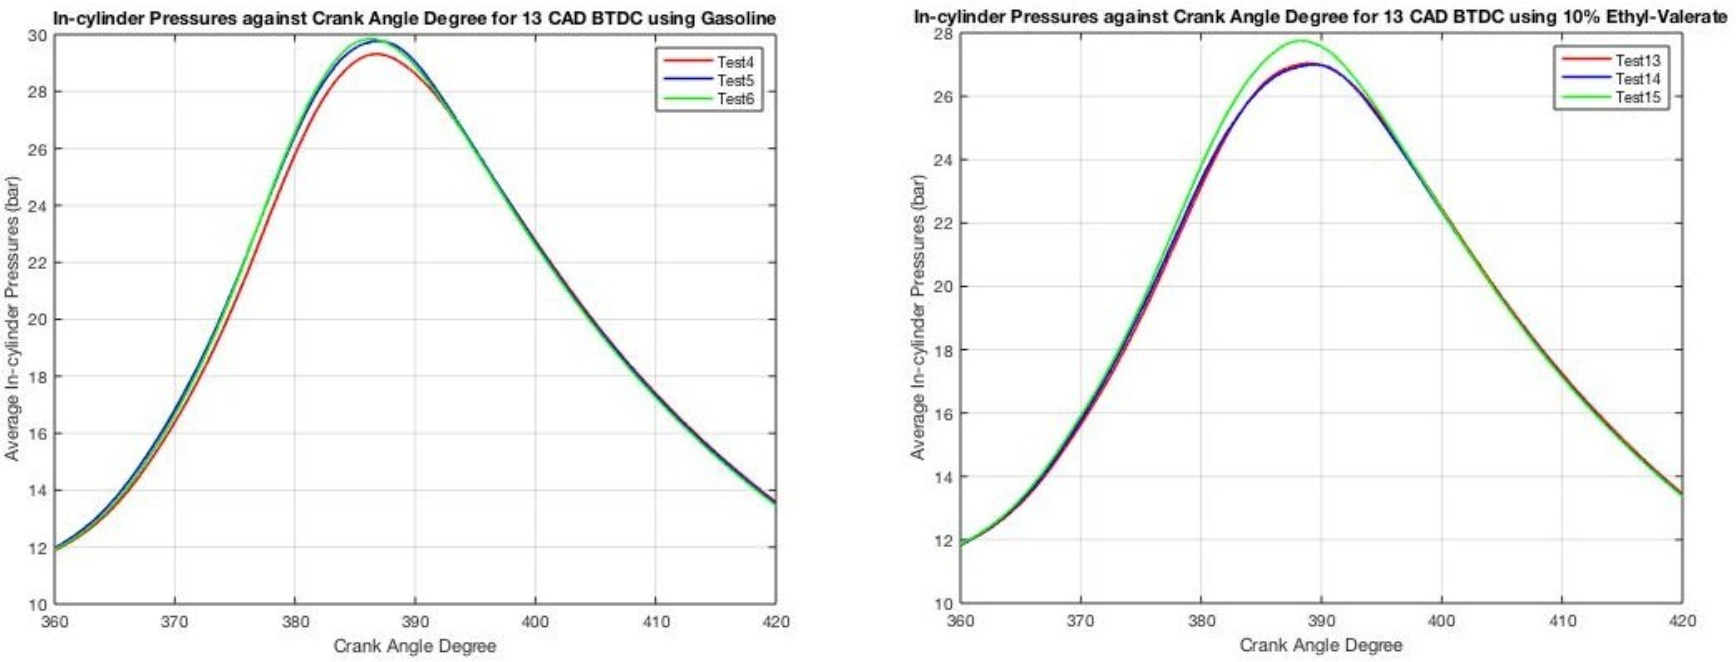
\includegraphics[width = \textwidth]{./img/diagram3.png}
    \caption{Variation of in-cylinder pressures against crank angle degree for both fuels.}
    \label{q5-f1}
\end{figure}
The three cycles show a variation in the instantaneous in-cylinder pressure cycles. The reason for the cycle-to-cycle variation in in-cylinder pressure is due to the variations in mixture motion, cyclic variations in the local equivalence ratio and the mixture composition near the spark plug. The air-fuel mixture might not be identical for every cycle that takes place which could create the variance in the pressure.  

There could be defects created during the manufacturing in the throttle valve of the engine or the defects could be due to wear, which would cause the intake of air-fuel mixture to be inconsistent, affecting the in-cylinder pressure. There could be a larger amount of intake, than what is required, into the combustion chamber which will cause the pressure to be irregular from cycle to cycle as we see the curves in Figure \ref{q5-f1} have different peaks. 

The vary in the speed of the engine could also have an effect on the in-cylinder pressure as in reality, the engine will not run at a constant speed due to discontinuities in flow, resistance and the change in momentum. Therefore, the time duration of the combustion cycle will change as the speed changes which will have an impact on the in-cylinder pressure during the cycle.  

Incomplete combustion of the fuel could be a reason for the change in in-cylinder pressure as unburnt fuel left over could affect the cycles after, causing the pressure in the cylinder to change as we get a varied amount of heat release in each cycle due to the inconsistency in the amount of fuel present for combustion. 

This cycle-to-cycle variations in in-cylinder pressure are not desirable as they lead to lower efficiency, limitations in power output and higher emissions. The varying pressure leads to varying amount of power output and this could affect the whole system as it may cause it to wear over time. This is due to the change in the pressure causing the components to experience a changing force which could cause damages. This varied power output limits performance and reliability of the engine.  
\section{Question 6}
Thermal engines present in modern cars rely on the combustion of fuel in oxygen to release energy \cite{q6-r1}. Ideally, this process should involve the complete combustion of all fuel with no excess oxygen; an air-fuel mixture containing the precise ratio of air to fuel required to ensure this is called a stoichiometric mixture. For a gasoline powered vehicle, this ratio is approximately 14.7:1 \cite{q6-r1}. It is important to maintain the air-fuel mixture in the combustion chamber of vehicles as close as possible to the ideal stoichiometric mixture as this ensures that the combustion process is most efficient, with the highest fuel economy and lowest emissions \cite{q6-r2}.

In fact, burning an air-fuel mixture that contains too much fuel and too little air (a rich mixture) will result in some of the fuel not being combusted, but released with the exhaust gases instead. This results in poor fuel economy as a portion of the fuel is wasted, as well as damage to the environment as the release of the unburned hydrocarbon fuels in the atmosphere will cause pollution. On the other hand, the combustion of a mixture that has too much oxygen/air and not enough fuel (a lean mixture) can have even more adverse consequences due to the increase in combustion chamber temperature that this process results in. The high temperatures can cause damage to the vehicle itself, e.g., damaging the pistons and spark plug, as well as promoting the production of Nitrous Oxides (\ce{NO_x})  which are remarkably damaging to the environment, as they are directly linked to smog and acid rain, and have indirect effects on human health, like causing breathing problems \cite{q6-r2} \cite{q6-r3} \cite{q6-r4}.

However, it is of relevance to mention that the stoichiometric ratio is not ideal for all operating conditions; in fact, when the vehicle is operating under a greater load, for instance, when it is accelerating, the engine is required to produce more power, thus a richer air-fuel mixture (a ratio between 13:1 and 12:1 for gasoline powered vehicles) which would produce more power should be burned instead \cite{q6-r4}. Thus, controlling and optimizing the air-fuel ratio is of vital importance for high engine performance and for maintaining high fuel economy as well as reducing emissions. It is the function of \ce{O2} sensors to monitor this ratio in modern cars by gauging the concentration of Oxygen in the exhaust gas (rather than the air-fuel mixture itself) and return this information to the Engine Control Unit (ECU) of the vehicle to control the ratio. 

\ce{O2} sensors are electronic transducers located in the exhaust pipe of vehicles. They are used to measure the proportion of Oxygen in the exhaust gas released by the vehicle and compare it to that measured in the atmospheric air in real time \cite{q6-r4}. These sensors are usually “solid-state electrochemical fuel cells […] that provide a certain output voltage depending on the amount of oxygen in the exhaust system relative to that in the atmosphere” \cite{q6-r4}. The sensor usually operates between two voltages (e.g., between \SI{0.2}{\volt} and \SI{0.8}{\volt} for narrowband sensors), the lower one associated with a lean mixture, the higher one with a rich mixture, and a middle voltage (\SI{0.45}{\volt} for narrowband sensors) associated with a nearly stoichiometric, optimal mixture \cite{q6-r4}. The output voltage, alongside with other sensors’ readings, is fed back to and processed by the ECU which automatically adjusts the air-fuel mixture as required by injecting more or less fuel into the mixture. The adjusted air-fuel mixture then undergoes combustion and releases new exhaust gases which will then be analysed by the \ce{O2} sensor and the process described above will continually repeat itself to maintain the ideal ratio. The use of this sensor permits closed loop operation of the air-fuel mixture – the information from the sensor is gathered and processed in real time, enabling the ECU to continuously change the air-fuel ratio, if needed, to match the desired one – ensuring optimal combustion conditions and engine function at all times.

In modern vehicles, \ce{O2} sensors are also used to measure the efficiency of catalytic converters. A catalytic converter is a device typically placed in the exhaust system of a vehicle that chemically changes some of the harmful gases (namely \ce{NO_x} and Carbon Monoxide) present in the exhaust gas of vehicle into more innocuous gases (Nitrogen, Carbon Dioxide and Water) in order to reduce exhaust emissions. By placing one oxygen sensor before the convertor and one after it, the difference in oxygen concentration between the gas that is yet to pass though the converter and the gas that has already passed through it can be measured, and this difference is used to assess the efficiency of the converter.
\section{Question 7}
\subsection*{Part A: Production}
A study published by the Royal Society of Chemistry shows that the esterification of valeric acid (VA) with ethanol catalysed by amino acid ionic liquids is a promising route of production for ethyl valerate (EV) \cite{q7-r1}. VA is obtained from cellulosic materials, a cheap and abundant renewable feedstock for biofuels which, importantly, does not compete with food supply like biofuels derived from starch-based plants.

Several amino acid ionic liquids can be used to catalyse the esterification process, including proline bisulfate (\ce{ProHSO4}), glycine bisulfate (\ce{GlyHSO4}), and alanine bisulfate (\ce{AlaHSO4}). The synthesis of these catalysts involves processes in water without by-products and post-processing, thus these preparations are highly efficient and low cost. 

The esterification process catalysed by \ce{ProHSO4} shows the most promise, with conversion rate above 99.9\% and 100\% selectivity for a 7-hour reaction at \SI{80}{\celsius}. As a comparison, the esterification process produced no EV in the absence of an acidic catalyst at room temperature and only 67\% of EV found using concentrated sulfuric acid at \SI{80}{\celsius}. The lipase process took up to 9 days to reach a conversion rate of 97.8\% and is thus much less efficient. 

The difference is due to the reaction mechanism. The reactants and ionic liquid catalyst are miscible in a single phase before reaction, but the produced EV has low solubility in the ionic liquid, resulting in a biphasic system, in which the unreacted VA and ethanol remained in the ionic liquid layer. Additionally, \ce{ProHSO4} acts as water absorbent since water as a by-product is also miscible in the ionic liquid layer, thus shifting the equilibrium of the reaction to the products without water removal. As a result, \ce{ProHSO4} facilitates the auto phase separation of the product from the reactants and by-products, favouring the conversion of VA and achieving a high EV yield, whilst restraining the reversible reaction of the ester. 

\ce{ProHSO4} is also easily recyclable from the products by a simple removal of water under vacuum taking place at \SI{100}{\celsius} for two hours. The reused catalyst showed similar catalytic performance to the original, with EV yield remaining above 95\% for five additional cycles of the reused catalyst.   

The sources of these lignocellulosic biomass from which VA is derived must also be considered when discussing EV as a potential biofuel. The revised Renewable Energy Directive (EU) 2018/2001 emphasizes the direct negative impact the procurement of biomass may have due to indirect land use change (ILUC). The production of biofuel may lead to the extension of agricultural land into areas with high carbon stock such as forests, wetlands and peatlands, the clearing of which may negate the positive effects of greenhouse gas savings from the increased use of biofuels \cite{q7-r2}. 

One way to mitigate the impact of ILUC is to produce lignocellulosic biomass from crop residues of agriculture, which does not require the extension of agricultural land. A study published in GCB Bioenergy estimated that in the reference period from 2011 to 2015, the total production of lignocellulosic material from crop residues in the EU28 is 419MT \cite{q7-r3}. From this estimate a sustained supply of crop residue for the production of biofuels can be deduced, though there are other important applications for crop residues, such as those related to soil quality and resilience.  

Additionally, the design of the supply chain is an important factor when considering the economic and environmental sustainability of our biofuel, of which the transportation of biomass plays a critical role. As such, the location of residue production within the EU28, the distance between production, processing and consumption hotspots, the timing of biomass supply, and the variability of crop yields year on year due to weather fluctuations are all critical factors to examine. Moreover, the GHG emissions during the transportation of the biomass must also be accounted for in the life cycle assessment of our biofuel.

In conclusion, ethyl valerate shows great promise of displacing gasoline if its production is catalysed by amino acid ionic liquids, namely proline bisulfate (\ce{ProHSO4}). The time and temperature of the production processes are relatively low whilst achieving conversion and selectivity of nearly 100\%. Ethanol is readily available, and the catalyst can be easily mass-produced due to the lack of post processing needed. Additionally, \ce{ProHSO4} is easily recyclable and can be reused multiple times with minimal impact on catalytic activity, improving its economic and environmental sustainability.

The main feedstock of lignocellulosic biomass, from which valeric acid is derived, is crop residues from agriculture and they are expected to play a major role in the production of advanced biofuels. Of course, valeric acid is not the only use of biomass both in the context of biofuel production and agricultural applications, though an optimised supply chain will increase the availability and decrease the cost of procurement. The design of the supply chain is a complicated process due to the factors mentioned previously, but also presents exciting opportunities, such as the densification of biomass with techniques such as baling, pelleting, and pyrolysis to reduce logistic costs \cite{q7-r4}. Ongoing research in this field and government incentives such as the EU’s Horizon 2020 program shows there is great potential for crop residues as a feedstock for lignocellulosic biomass.
\subsection*{Part B: Efficiency and emissions}
The efficiency and emissions of the ethyl valerate test fuel blend must also be examined to better judge its suitability in replacing gasoline. For all spark timings investigated, the thermal efficiency of the ethyl valerate test fuel blend was higher when compared to gasoline (see Figure \ref{q3-f2}). This is caused by the lower indicated specific fuel consumption using the test fuel blend at all spark timing when compared to gasoline (not including test 4). This result is slightly unexpected given the higher energy density of gasoline, meaning the ISFC of gasoline should be lower.

The reason for this is likely to be the narrow range of spark timings investigated. As previously mentioned, experimental data has shown 31 CAD BTDC to be the optimal spark timing for the combustion of gasoline in a spark ignition engine. If the range of spark timings investigated were to be increased, we would likely see a range of spark timings across which the ISFC of gasoline was higher than the test fuel blend, leading to higher thermal efficiencies. 

For all spark timings investigated, the emissions of both \ce{CO2} and \ce{NO_x} were lower for the test fuel blend when compared to gasoline. Additionally, the emissions of both gases were lower for earlier spark timings when using the test fuel blend; whilst the opposite was true for gasoline, emissions were higher for earlier spark timings.

The difference in the amount of \ce{CO2} produced can be explained by the chemical composition of the fuels. Since gasoline, whose main component is octane (\ce{C8H18}), is more carbon heavy than ethyl valerate (\ce{C7H14O2}), thus blending ethyl valerate with gasoline will reduce the carbon dioxide produced during combustion. Similarly, since more air is required for the combustion of air with gasoline than the test fuel blend, more \ce{NO_x} is produced since the formation of it is highly oxygen dependent. 

Interestingly, temperature and fuel viscosity dependence seem to have little effect on the \ce{NO_x} emissions. Theoretically, \ce{NO_x} emissions increase with both increasing combustion temperature and fuel viscosity. Table \ref{q7-t1} shows that for all spark timings, the exhaust gasses are hotter for the test blend when compared to gasoline, which suggest combustion temperatures are higher. Furthermore, the test blend had a much higher viscosity of \SI{1.08}{\milli\pascal\second} compared to \SI{0.61}{\milli\pascal\second} for gasoline.

\begin{table}[H]
	\begin{center}
	\begin{tabular}{@{}lll@{}}
		\toprule
		Spark Timing & \multicolumn{2}{c}{Average Exhaust Gas Temperature (Celsius)} \\
		\cmidrule{2-3} & 10\% Ethyl Valerate & Reference Gasoline \\
		\midrule
		10 CAD BTDC & 477.7 & 461.1 \\
		13 CAD BTDC & 492.7 & 481.0 \\
		16 CAD BTDC & 493.3 & 484.3 \\
		\bottomrule
	\end{tabular}
	\caption{Average exhaust gas temperature for all spark timings.}
	\label{q7-t1}
	\end{center}
\end{table}
Both factors suggest that \ce{NO_x} emissions should be higher for the ethyl valerate test blend, though we do not observe this in our data. Again, it is important to note the narrow range of spark timings across which our results were collected. Plotting \ce{NO_x} emissions against spark timing (see FIGURE X) suggest that \ce{NO_x} emissions for ethyl valerate will increase beyond the \ce{NO_x} emissions for gasoline, which looks to have reached a maximum near 10 CAD BTDC. However, these trends are by no means conclusive and must be tested experimentally.
\section{Conclusions}
Based on this study, we can make observations about the performance of spark ignition engines as the spark timing is varied. It is seen that an earlier spark timing results in higher IMEP, and therefore higher thermal efficiency (assuming no variability in combustion conditions). However this is known to be at the expense of higher NOx emissions, which are toxic to human health, and the emergence of engine knock, which causes premature wear on the components. These are all an effect of the higher temperatures in the cylinder. As a result, increasing thermal efficiency by bringing ignition earlier must be balanced with these effects in mind. 

The indicated thermal efficiency for all test conditions were about 30\%. We see that in the conversion of heat energy from the chemical energy released in burning of the fuel to work in the engine, a large amount of the heat energy is lost as waste heat.

Some conclusions may also be drawn between the two different fuels used. The Ethyl Valerate blend performed better than gasoline at all spark timings both in terms of thermal efficiency and pollutant emissions. However, due to the narrow range of spark timings investigated, the test fuel blend cannot conclusively be recommended as a potential replacement for gasoline. At different spark timings, gasoline may outperform the test fuel blend. The analysis would also benefit from data about additional pollutants such as unburnt fuel, carbon monoxide, and particulates. Furthermore, efficiency and emissions are not the only parameters to be examined. For example, for power sensitive applications such as high-performance vehicles, IMEP is a much more important parameter to consider. Overall, the performance the Ethyl Valerate test fuel blend shows promise, though much more data would be needed to make a definitive judgement. 
\begin{thebibliography}{00}
\bibitem{i1} Public Health England, "Health Matters: air pollution" 14 Nov 2018, URL: \url{https://www.gov.uk/government/publications/health-matters-air-pollution/health-matters-air-pollution#:~:text=Poor%20air%20quality%20is%20the,leading%20to%20reduced%20life%20expectancy.} [Accessed 26 March 2021]
\bibitem{r0} Talibi, M., Hellier, P., \textit{MECH0011: Combustion characteristics of a spark ignition engine operated with renewable fuels} Introductory Lecture.
\bibitem{q1-r1} Zareei, J. and Kakaee, A., 2013. Study and the effects of ignition timing on gasoline engine performance and emissions. European Transport Research Review, [online] 5(2), pp.109-116. Available at: \url{https://link.springer.com/content/pdf/10.1007\%2Fs12544-013-0099-8.pdf} [Accessed 22 March 2021]. 
\bibitem{q1-r2} Manofsky, L., Vavra, J., Assanis, D., Babajimopoulos, A., (2011). ``Bridging the gap between HCCI and SI: Spark-assisted compression ignition''. SAE Technical Paper Series. 
\bibitem{q2-r1} PubChem. 2021. PubChem Compound Summary for CID 10882, Ethyl valerate. [online] Available at: \url{https://pubchem.ncbi.nlm.nih.gov/compound/Ethyl-valerate} [Accessed 22 March 2021]. 
\bibitem{q2-r2} PubChem. 2021. PubChem Compound Summary for CID 356, Octane. [online] Available at: \url{https://pubchem.ncbi.nlm.nih.gov/compound/octane} [Accessed 22 March 2021]. 
\bibitem{q2-r3} Hellier, P., 2013. The Molecular Structure of Future Fuels. [online] Available at: \url{https://core.ac.uk/download/pdf/16253499.pdf} [Accessed 22 March 2021]. 
\bibitem{q3-r1} Lopes, S.M., Furey, R., Geng, P., 2013. Calculation of Heating Value for Diesel Fuels Containing Biodiesel. SAE International Journal of Fuels and Lubricants, Vol. 6, No. 2, pp. 407-418 [online]. Available at: \url{https://www.jstor.org/stable/26273015} [Accessed 15 March 2021]. 
\bibitem{q3-r2} Luo, K., 2021. Lecture 4: Elementary Combustion.  
\bibitem{q3-r3} NIST Chemistry WebBook. n.d. Pentanoic acid, ethyl ester. [online] Available at: \url{https://webbook.nist.gov/cgi/cbook.cgi?ID=C539822&Mask=1EFF} [Accessed 15 March 2021]. 
\bibitem{q3-r4} Moran, M. and Shapiro, H., 2014. Fundamentals of Engineering Thermodynamics. 8th ed. Wiley. 
\bibitem{q3-r5} Stone, R., 1992. Introduction to Internal Combustion Engines. 2nd ed. Basingstoke, England: Macmillan, pp.24-26.  
\bibitem{q4-r1}The Engineering Toolbox. n.d. ``Water - Specific Heat''. [online] Available at: \url{https://www.engineeringtoolbox.com/specific-heat-capacity-water-d_660.html}
\bibitem{q4-r2} Parthasarathi, B., (2010) ``Recent advances in auto exhaust catalysis''. Journal of the Indian Institute of Science, 90(2). [online] Available at: \url{https://www.researchgate.net/publication/233532567_Recent_advances_in_auto_exhaust_catalysis}
\bibitem{q4-r3} The Engineering Toolbox. n.d. ``Water Vapour - Specific Heat''. [online] Available at: \url{https://www.engineeringtoolbox.com/water-vapor-d_979.html}
\bibitem{q4-r4} VW, S.B. n.d. MIT OCW. 3.5 The internal combustion engine (Otto Cycle). [online] Available at: \url{https://web.mit.edu/16.unified/www/FALL/thermodynamics/notes/node26.html}
\bibitem{q6-r1}X-engineer.org. n.d. ``Air-fuel ratio, lambda and engine performance''. [online] Available at: \url{https://x-engineer.org/automotive-engineering/internal-combustion-engines/performance/air-fuel-ratio-lambda-engine-performance/}
\bibitem{q6-r2} Haynes Publishing. n.d. ``What is AFR, or Air/Fuel Ratio, in your car?''. [online] Available at: \url{https://haynes.com/en-gb/tips-tutorials/what-afr-or-airfuel-ratio-your-car}
\bibitem{q6-r3} Phys.org. 2015. ``NOx gases in diesel car fumes: Why are they so Dangerous?''. [online] Available at: \url{https://phys.org/news/2015-09-nox-gases-diesel-car-fumes.html#:~:text=NOx\%20has\%20direct\%20and\%20indirect,of\%20appetite\%20and\%20corroded\%20teeth} 
\bibitem{q6-r4} Goodfabs.com. 2020. Oxygen sensors and engine power. [online] Available at: \url{https://www.goodfabs.com/post/how-oxygen-sensors-work}
\bibitem{q7-r1} Dong, L-L., He, L., Tao, G-H., et al. (2013). ‘High yield of ethyl valerate from the esterification of renewable valeric acid catalyzed by amino acid ionic’. RSC Advances, 14 (April), pp. 4457-4836. doi: 10.1039/c3ra23034a]
\bibitem{q7-r2} European Commission (2020).  Sustainability criteria. [online] Available at: \url{ec.europa.eu/energy/topics/renewable-energy/biofuels/sustainability-criteria_en?redir=1} (Accessed: 23 March. 2021)
\bibitem{q7-r3} Garcia-Condado, S., Lopez-Lozano, L., Panarello, L., et al. (2019) ``Accessing lignocellulosic biomass production from crop residues in the European Union: Modelling, analysis of the current scenario and drivers of interannual variability''. GCB Bioenergy, 11(6), pp. 809-831. doi: doi.org/10.1111/gcbb.12604
\bibitem{q7-r4} Albashabsheh, N., Heier Stamm, J. (2021) ‘Optimization of lignocellulosic biomass-to-biofuel supply chains with densification: Literature review’. Biomass and Bioenergy, 144. doi: doi.org/10.1016/j.biombioe.2020.105888
\end{thebibliography}
\end{document}
